\documentclass[thesis.tex]{subfiles}

\begin{document}

\chapter{Additional plots for \cref{E-transmission}}

\begin{figure}
    \thisfloatpagestyle{empty}
    \vspace{-3cm}
    \makebox[\textwidth][c]{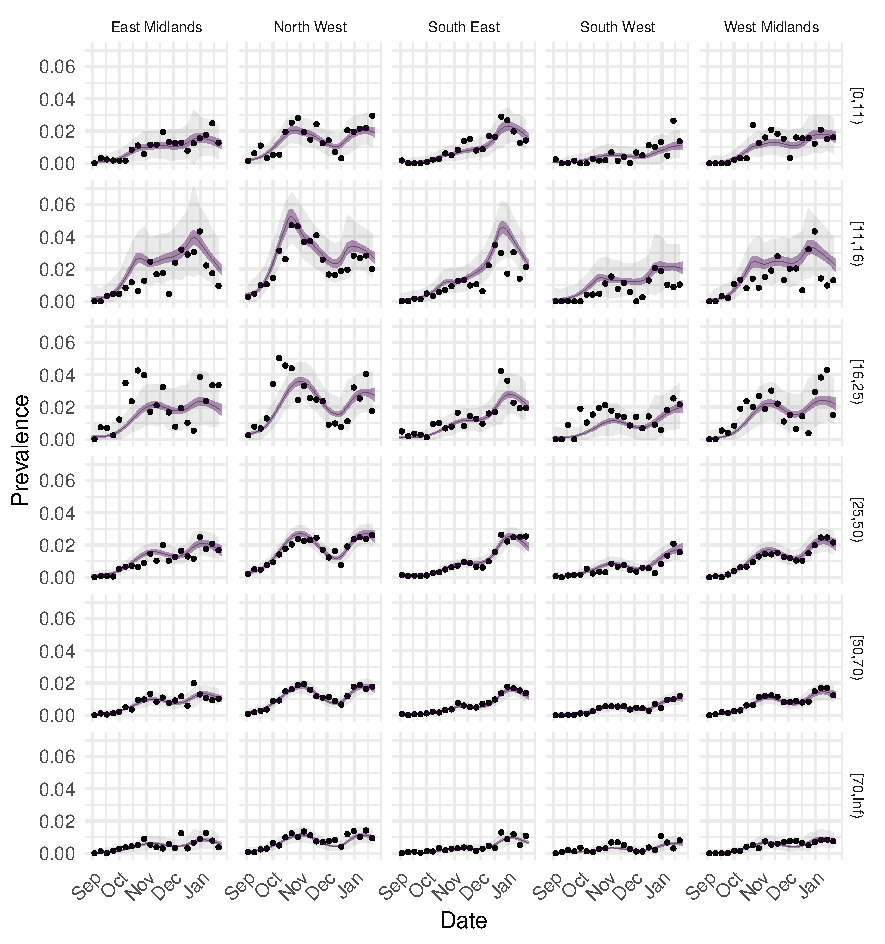
\includegraphics[width=.9\paperwidth]{SEIR/CIS/prev_appendix}}
    \captionsetup{width=0.8\paperwidth}
    \captionof{figure}[Other SEIR prevalence goodness-of-fit]{%
        Goodness-of-fit to prevalence data by region and age for selected regions (see \cref{SEIR:fig:prev} for others).
        The central ribbon and line show the posterior median and 95\% CrI estimate for the proportion of the relevant stratum RT-PCR positive on each day.
        The lighter outer ribbon is the 95\% posterior predictive interval for the proportion of test results that are positive each week.
        The dots show the observed prevalence in CIS, aggregated by week.
        For a well-calibrated model, 95\% of the dots would be within the outer ribbon.
    }
    \label{SEIR:fig:prev-appendix}
\end{figure}

\end{document}